\chapter{Research plan}
In order to achieve the research and educational objectives of this project, in this chapter the expected time line to be followed, the list of planned publications and the list of courses to attend are presented. 



\section{Time plan}
The time line below shows the set of activities to be pursued during the project and when they will be happening. The time line shows that some of the activities in the project are needed to be executed in parallel and some other require inputs from previous stages to be completed. The second part of the table shows what are academic articles to be delivered as the project progresses. \par
Following the stages above, during the first year the domain of research and the research questions were defined. This was possible as a result of background readings on different fields and realizing a knowledge gap a need from policy makers and practitioners to spatialize the concepts of circular economy. The second year will be focused on developing a general framework and data model that will allow in the follow up stages of the research to evaluate scenarios, describe an urban system in terms of waste management (municipal or industrial) and study its performance. 
The table below details the tasks that will be executed in the future. \par

\begin{figure}[h!]
    \centering
    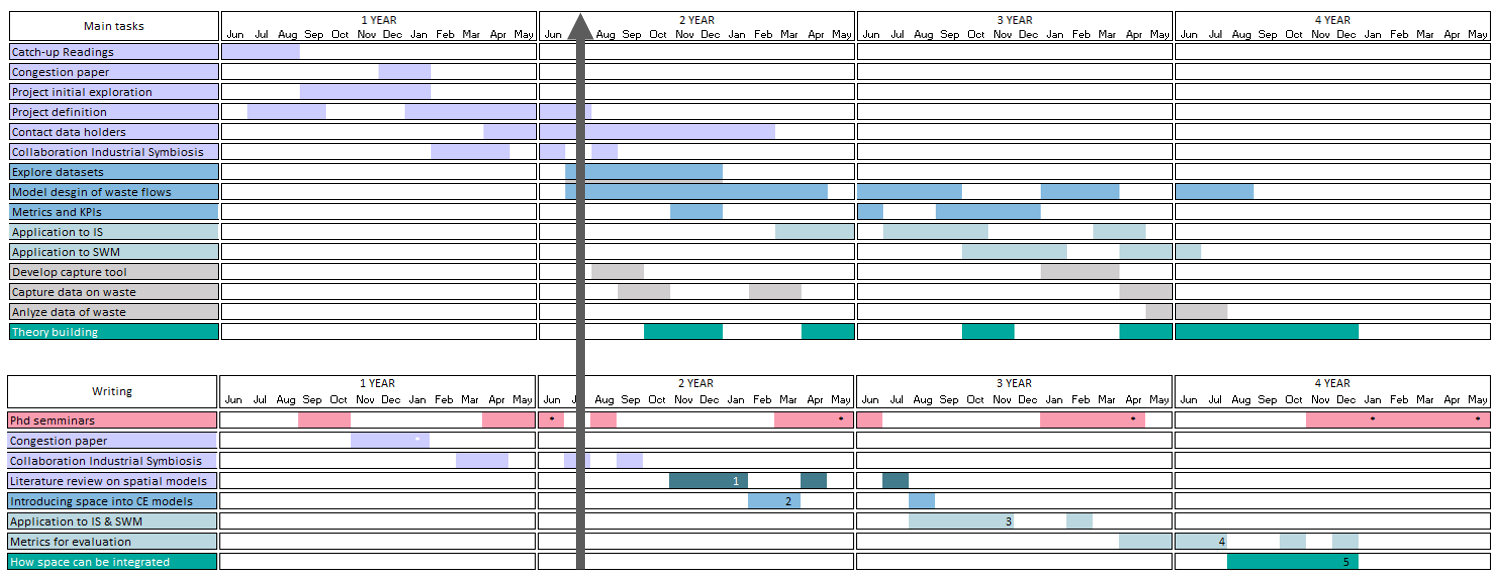
\includegraphics[width=0.95\textwidth]{sections/asset/timeplan.PNG}
    \caption{Time plan for the research proposal}
    \label{fig:research_time}
\end{figure}


The second part of the diagram shows what stages will be related to what publications. This is the list of publications suggested: 



\subsubsection{2020. Literature review of how space is integrated in waste flows models}


\subsubsection{2020. Make a first data model proposition of how to integrate space in a general model}


\subsubsection{2021. Application to IS \& solid waste management}


\subsubsection{2021. Metrics to evaluate circular economy}


\subsubsection{2022. Importance of regional planning to promote IS and better solid waste management systems}


\subsubsection{2022. Data capturing and feeding the data model. An illustration} 



% \section{Deliverable}



% \section{Doctoral education}

% \subsection{GTS - Mandatory}

% \begin{enumerate}
%     \item [DONE] Sustainable development: values, technology in society, and the researcher GFOK105 • 3 HEC
%     \item [DONE] General introduction for doctoral students GFOK015 • 0 HEC
%     \item [DONE] Career planning - your personal leadership GFOK010 • 1,5 HEC
%     \item [After Lic] Teaching, learning and evaluation GFOK020 • 3 HEC
%     \item [After Lic] Popular science presentation GFOK070 • 0 HEC
% \end{enumerate}

% \subsection{GTS}

% %\begin{enumerate}
% %    \item 
% %\end{enumerate}

% \subsection{Topic specific}

% \begin{enumerate}
%     \item Urban Metabolism \& resources
%     \item Industrial Ecology
%     \item 
% \end{enumerate}







